\documentclass[12pt, a4paper, twoside, openright]{Thesis} % Paper size, default font size and one-sided paper
\usepackage[utf8]{inputenc}
\usepackage{wrapfig}
\usepackage{lscape}
\usepackage{rotating}
\usepackage{graphicx}
\usepackage{caption}
\usepackage{amsmath, nccmath}
\usepackage{comment}
\usepackage{afterpage}
\usepackage{multirow}
\usepackage{multicol}
\usepackage{cleveref}
\usepackage{rotating}
\usepackage[font=small]{caption}
% \captionsetup{compatibility=false}
\usepackage{subcaption}
% \usepackage{subfig}
\usepackage{makecell}
\usepackage{booktabs}
\usepackage{multirow}
\usepackage{lscape}
\usepackage{longtable}
\usepackage{placeins}
\usepackage{adjustbox}
\usepackage{enumitem} % for roman letter lists
\usepackage{amssymb}
\usepackage{afterpage}
\usepackage{lipsum}
\usepackage{listings}

% Tikz library
\usepackage{tikz}
\usetikzlibrary{shapes.geometric, arrows}

% Defining Tickz Style
\tikzstyle{startstop} = [rectangle, rounded corners, minimum width=3cm, minimum height=1cm, text centered, text width = 6cm, draw=black, fill=white]

\tikzstyle{startstop1} = [rectangle, rounded corners, minimum width=3cm, minimum height=1cm, text centered, draw=black, fill=white]

\tikzstyle{io} = [trapezium, trapezium left angle=70, trapezium right angle=110, minimum width=3cm, minimum height=1cm, text centered, text width = 4.5cm, draw=black, fill=blue!30]

\tikzstyle{process} = [rectangle, minimum width=3cm, minimum height=1cm, text centered, text width = 6cm, draw=black, fill=orange!30]

\tikzstyle{decision} = [diamond, minimum width=3cm, minimum height=1cm, text centered, draw=black, fill=green!30]

\tikzstyle{arrow} = [thick,->,>=stealth]

% Gentt Chart
\usepackage{pgfgantt}
\usepackage{xcolor}

% \usepackage[dvipsnames]{xcolor}
\newcommand\myemptypage{
    \null
    \thispagestyle{empty}
    \addtocounter{page}{-1}
    \newpage
    }
    

%\usepackage[width=14cm, left=3cm]{geometry}

% prints author names as small caps


%\usepackage{subcaption} %incompatible with subfig
\graphicspath{{Pictures/}} % Specifies the directory where pictures are stored
\usepackage[authoryear]{natbib}
%\usepackage[square, numbers]{natbib} % Use the natbib reference package - read up on this to edit the reference style; if you want text (e.g. Smith et al., 2012) for the in-text references (instead of numbers), remove 'numbers' v
%\bibliographystyle{abbrvnat}
%\setcitestyle{authoryear,open={((},close={))}}
\hypersetup{colorlinks=true, linkcolor={blue}, citecolor={blue}, urlcolor={blue}} % Colors hyperlinks in blue - change to black if annoyingv`	
\title{\ttitle} % Defines the thesis title - don't touch this

\begin{document}
% \makeatletter
% \renewcommand*{\NAT@nmfmt}[1]{\textsc{#1}}
% \makeatother

% prints author names as small caps
% it is sometimes necessary in user documents to have access to such package-internal macros, and so the commands \makeatletter and \makeatother change the catcode

\frontmatter % Use roman page numbering style (i, ii, iii, iv...) for the pre-content pages

\setstretch{1.6} % Line spacing of 1.6 (double line spacing)

% Define the page headers using the FancyHdr package and set up for one-sided printing
\fancyhead{} % Clears all page headers and footers
\rhead{\thepage} % Sets the right side header to show the page number
\lhead{} % Clears the left side page header

\pagestyle{fancy} % Finally, use the "fancy" page style to implement the FancyHdr headers

\newcommand{\HRule}{\rule{\linewidth}{0.5mm}} % New command to make the lines in the title page

% PDF meta-data
\hypersetup{pdftitle={\ttitle}}
\hypersetup{pdfsubject=\subjectname}
\hypersetup{pdfauthor=\authornames}
\hypersetup{pdfkeywords=\keywordnames}

%----------------------------------------------------------------------------------------
%	TITLE PAGE
%----------------------------------------------------------------------------------------
\begin{comment}
\begin{titlepage}
\begin{center}

\HRule \\[0.4cm] % Horizontal line
{\huge \bfseries \ttitle}\\[0.4cm] % Thesis title
\HRule \\[1.5cm] % Horizontal line
 
\large \textit{A thesis submitted in fulfilment of the requirements\\ for the degree of \degreename}\\[0.3cm] % University requirement text
\textit{by}\\[0.4cm]

%\href{http://home.iitk.ac.in/~saiwal}{\authornames}

\vfill
\graphicspath{ {./Figures/} }
\begin{figure}[hb]
  \centering
  \includegraphics[width=0.4\linewidth]{Images/redlogo.png}
\end{figure}

\DEPTNAME\\ % Research group name and department name
\textsc{ \UNIVNAME}\\[1.5cm] % University name
\large \today\\[2cm] % Date


\end{center}

\end{titlepage}
\end{comment}
%\begin{document}
\begin{titlepage}


%\newgeometry{centering,top = 2.54cm,bottom = 2.54cm,left = 2.54cm, right = 2.54cm, includeheadfoot}

\pagenumbering{gobble}% Remove page numbers (and reset to 1)
\thispagestyle{empty}
\singlespacing
\begin{titlepage}
%\setlength{\voffset}{-0.1in}
%\setlength{\headsep}{5pt}
%\setlength{\textheight}{650pt}
%titlepage
%\thispagestyle{empty}
\begin{center}
%\begin{minipage}{0.75\linewidth}
    \centering
     
%=====================================================%
%---------------THESIS TITLE--------------------------%
%=====================================================%    
\definecolor{blue}{rgb}{0,0,1} % before using a colour one has to define it like this, here you have given color with rgb as 0,0,1 as blue
\definecolor{black}{rgb}{0,0,0} % before using a colour one has to define it like this, here you have given color with rgb as 0,0,1 as blue
      
  {{\Large \textbf{Enhancing Trust and Traceability in Supply Chains 
  through Blockchain and Machine Learning}\par}}
    \vspace{1cm}% FOR CREATING DESIRED SPACE BETWEEN THE LINES
     
%=====================================================%
%---------------Partial Fulfillment---------------------%
%=====================================================%
    \vspace{0.4cm}
    {
    \textbf{\large Project report submitted for the requirement for the degree of } \par}
    \vspace{0.2cm}

%=====================================================%
%---------------Degree---------------------%
%=====================================================%

\vspace{0.5cm}
    {
    \textbf{\large Bachelor of Technology \\ \vspace{1mm} } \par}
    \vspace{2mm}


    

%=====================================================%
%---------------AUTHOR'S NAME-------------------------%
%=====================================================%
\vspace{5mm}
    {\large by\par}
    \vspace{0.05cm}
    {\large \textbf{\textcolor{black}{Jivanjyoti Bhattacharaya}}  (190710007028)\par} 
    {\large \textbf{\textcolor{black}{Dipjyoti Kashayp}}  (200750007002)\par} 
    {\large \textbf{\textcolor{black}{Hema Gohain}}  (200750007003)\par} 
    {\large \textbf{\textcolor{black}{Tajkiratul Qubra}}  (200750007007)\par} 
%    {\Large \textbf{(2013MEZ8469)}\par}
    \vspace{0.4cm}
    
%=====================================================%
%---------------Supervisor Name---------------------%
%=====================================================%    
%    {\Large \textbf{Doctor of Philosophy} \par}
%    \vspace{0.5cm}
    { Under the Supervision of \par}
    {\large \textbf{\textbf{\textcolor{black}{Rajib Chakrabarty}}}\par}
%    {\Large \textbf{(2013MEZ8469)}\par}
     \vspace{0.8 cm}

%=====================================================%
%---------------UNIVERSITY lOGO-----------------------%
%=====================================================%

\includegraphics[width=0.25\linewidth]{Images/jec_logo.png}
%    \rule{0.4\linewidth}{0.15\linewidth}\par
     \vspace{0.6 cm}

    
%=====================================================%
%---------------DEPARTMENT'S NAME-------------------------%
%=====================================================%
    {\large Department of Computer Science \& Engineering\par}
    \vspace{0.4cm}

    {\large \textbf{Jorhat Engineering College}\par}
    \vspace{0.4cm}
%=====================================================%
%---------------DATE----------------------------------%
%=====================================================%
    {\large \textbf{Jorhat - 785007, India}}
    \vspace{0.4cm}
    
    % {\large {May, 2025}}
%\end{minipage}
\end{center}
\end{titlepage}
\end{titlepage}
% \myemptypage
%\afterpage{\null\newpage}
%\include{blank_page_1}
%\newpage
% \newpage
% %\newgeometry{centering,top = 2.54cm,bottom = 2.54cm,left = 2.54cm, right = 2.54cm, includeheadfoot}

\pagenumbering{gobble}% Remove page numbers (and reset to 1)
\thispagestyle{empty}
\singlespacing
\begin{titlepage}
%\setlength{\voffset}{-0.1in}
%\setlength{\headsep}{5pt}
%\setlength{\textheight}{650pt}
%titlepage
%\thispagestyle{empty}
\begin{center}
%\begin{minipage}{0.75\linewidth}
    \centering
     
%=====================================================%
%---------------THESIS TITLE--------------------------%
%=====================================================%    
\definecolor{blue}{rgb}{0,0,1} % before using a colour one has to define it like this, here you have given color with rgb as 0,0,1 as blue
      
  {{\Large \textbf{Smart Supply Chain}\par}}
    \vspace{1cm}% FOR CREATING DESIRED SPACE BETWEEN THE LINES
     
%=====================================================%
%---------------Partial Fulfillment---------------------%
%=====================================================%
    \vspace{0.4cm}
    {
    \textbf{\large A Credit Seminar Report (CE694)} \par}
    \vspace{0.2cm}

%=====================================================%
%---------------Degree---------------------%
%=====================================================%

\vspace{0.5cm}
    {
    \textbf{\large Master of Technology\\ \vspace{1mm} in\\ \vspace{1mm}  Transportation Systems Engineering} \par}
    \vspace{2mm}


    

%=====================================================%
%---------------AUTHOR'S NAME-------------------------%
%=====================================================%
\vspace{5mm}
    {\large by\par}
    \vspace{0.05cm}
    {\large \textbf{\textcolor{blue}{Your Name}} \\ (22xxxxx)\par} 
%    {\Large \textbf{(2013MEZ8469)}\par}
    \vspace{0.4cm}
    
%=====================================================%
%---------------Supervisor Name---------------------%
%=====================================================%    
%    {\Large \textbf{Doctor of Philosophy} \par}
%    \vspace{0.5cm}
    { Under the Supervision of \par}
    {\large \textbf{\textbf{\textcolor{blue}{Prof. Name}}}\par}
%    {\Large \textbf{(2013MEZ8469)}\par}
     \vspace{0.8 cm}

%=====================================================%
%---------------UNIVERSITY lOGO-----------------------%
%=====================================================%

\includegraphics[width=0.25\linewidth]{Images/jec_logo.png}
%    \rule{0.4\linewidth}{0.15\linewidth}\par
     \vspace{0.6 cm}

    
%=====================================================%
%---------------DEPARTMENT'S NAME-------------------------%
%=====================================================%
    {\large Department of Civil Engineering\par}
    \vspace{0.4cm}

    {\large \textbf{INDIAN INSTITUTE OF TECHNOLOGY BOMBAY}\par}
    \vspace{0.4cm}
%=====================================================%
%---------------DATE----------------------------------%
%=====================================================%
    {\large \textbf{Mumbai - 400076, India}}
    \vspace{0.4cm}
    
    {\large {May, 2025}}
%\end{minipage}
\end{center}
\end{titlepage}
% \newpage
% \myemptypage

%----------------------------------------------------------------------------------------
%	DEDICATION
%----------------------------------------------------------------------------------------
%
\setstretch{1.3} % Return the line spacing back to 1.3
%
\pagestyle{empty} % Page style needs to be empty for this page
%
% \dedicatory{\textit{Dedicated to Road Crash Victims}} % Dedication text
% %
% \addtocontents{toc}{\vspace{2em}} % Add a gap in the Contents, for aesthetics
% \newpage


%-------------------------------------------------------------
%	DECLARATION PAGE
%	Your institution may give you a different text to place here
%----------------------------------------------------------------------------------------

% \Declaration{\addtocontents{toc}{\vspace{1em}} % Add a gap in the Contents, for aesthetics

% This is to certify that the thesis entitled \textbf{``Study of Pedestrians’ Unsafe Road Crossing Behaviour at Signalised Intersection Crosswalks''}, submitted by \textbf{Rahul Raoniar} [Roll No. 166104036], to the Indian Institute of Technology Guwahati, for the award of the degree of \textbf{Doctor of Philosophy} in Transportation Systems Engineering, is a record of the original, bona fide research work carried out by him under my supervision and guidance. The thesis has reached the standards fulfilling the requirements of the regulations related to the award of the degree.

% \par The results contained in this thesis have not been submitted in part or in full to any other University or Institute for the award of any degree or diploma to the best of our knowledge.
% \bigskip
% \bigskip
% \bigskip
% \bigskip


% \vspace*{2.5cm} %\vfill
% % \begin{multicols}{2}
% % \begin{center}
% \begin{flushleft}
% % \begin{center}
% \hspace{1.8mm} \textbf{Prof. Akhilesh Kumar Maurya}\\
% \hspace{3.2mm} Department of Civil Engineering\\
% Indian Institute of Technology Guwahati
% % \end{center}
% \end{flushleft}

% \end{center}
% \begin{center}
%\begin{flushleft}
%Date:
%\end{flushleft}
% \textbf{Prof. XXXXXXXXXXX XXXXXXXX}\\
% Department of XXXXXXXX,\\
% Indian Institute of Technology Guwahati.
% \end{center}
% \end{multicols}
% \vfill{}}

% \clearpage % Start a new page


% % Addded a Declaration statement page


% \addtotoc{Declaration} % Add the "Scope for future work" page entry to the Contents

% {\addtocontents{toc}{\vspace{1em}} % Add a gap in the Contents, for aesthetics

% \centerline{\textbf{\LARGE {Declaration}}}}
% \vspace{3em}
% I declare that this written submission represents my ideas in my own words, and where others' ideas and words have been included, I have adequately cited and referenced the original source. I declare that I have adhered to all principles of academic honesty and integrity and have not misrepresented or fabricated, or falsified any idea/data/fact/source in my submission. I understand that any violation of the above will cause disciplinary action by the Institute and can also evoke penal action from the source which has thus not been properly cited or from whom proper permission has not been taken when needed.

% \bigskip
% \bigskip
% \bigskip
% \bigskip

% \ldots \ldots \ldots \ldots \ldots \ldots \\
% \vspace{2mm}
% \textbf{Rahul Raoniar} \\
% Roll No.: 166104036 \\
% Date: \\
% Place: Guwahati

% \clearpage % Start a new page

%----------------------------------------------------------------------------------------
%	ACKNOWLEDGEMENTS
%----------------------------------------------------------------------------------------

\setstretch{1.3} % Reset the line-spacing to 1.3 for body text (if it has changed)

% \acknowledgements{\addtocontents{toc}{} % Add a gap in the Contents, for aesthetics
\acknowledgements{{} % Add a gap in the Contents, for aesthetics


We would like to express our deep sense of gratitude and special thanks to our guide, \textbf{Rajib Chakrabarty} who not only took a great interest in the project but also was always ready 
to help us as and when needed. \par We are also grateful to \textbf{Dr. Rupam Baruah} (Head of Computer \& Science  Engineering Department) and all staff members of the Computer Science \&  Engineering Department for their kind co-operation. \\ Finally, we are thankful to all our friends who have helped for presenting \& preparation of our project.


\textbf{Jivanjyoti Bhattacharayya (190710007028)}\\
\textbf{Dipjyoti Kashayp (200750007002)}\\
\textbf{Hema Gohain (200750007003)}\\
\textbf{Tajkiratul Qubra (200750007007)}

}
% \clearpage % Start a new page

\newpage
% \myemptypage

\clearpage % Start a new page
%----------------------------------------------------------------------------------------
%	ABSTRACT PAGE
%----------------------------------------------------------------------------------------

% \addtotoc{Certificate} % Add the "Abstract" page entry to the Contents
\certificate{\addtocontents{toc}{} % before using a colour one has to define it like this, here you have given color with rgb as 0,0,1 as blue
      
 
%\noindent
This is to certify that this project entitled \textbf{Enhancing Trust and Traceability in Supply Chains 
through Blockchain and Machine Learning} is done by \textbf{JIVANJYOTI BHATTACHARYYA},
\textbf{DIPJYOTI KASHYAP}, \textbf{HEMA GOHAIN} and \textbf{TAJKIRATUL QUBRA} Roll No 
\textbf{190710007028},\textbf{ 200750007002},\textbf{ 200750007003} and \textbf{200750007007} . Under the guidance and 
supervision in a benefited student of the Department of Computer Science \& Engineering has 
carried this project as fulfillment of the requirement of a B.tech in Computer Science \& 
Engineering and this work is presented in this report has presented for academic purpose. 

% \textbf{RAJIB CHAKRABARTTY}          \textbf{DIGANTA BAISHYA}\par      
\textbf{\makebox[0.5\textwidth][l]{RAJIB CHAKRABARTTY}\hfill\makebox[0.5\textwidth][r]{Dr. RUPAM BARUAH}} 
\textbf{\makebox[0.5\textwidth][l]{Guide}\hfil\makebox[0.5\textwidth][r]{HOD,CSE}}
% \textbf{GUIDR}
% \textbf{GUIDR}\par
Place- Jorhat\par
Date:- 26/06/2023
}

\newpage
% \myemptypage

\clearpage % Start a new page
%----------------------------------------------------------------------------------------
%	ABSTRACT PAGE
%----------------------------------------------------------------------------------------

% \addtotoc{Certificate} % Add the "Abstract" page entry to the Contents
\certificate{\addtocontents{toc}{} % before using a colour one has to define it like this, here you have given color with rgb as 0,0,1 as blue
      
 
%\noindent
This is to certify that this project entitled \textbf{Enhancing Trust and Traceability in Supply Chains 
through Blockchain and Machine Learning} is done by \textbf{JIVANJYOTI BHATTACHARYYA},
\textbf{DIPJYOTI KASHYAP}, \textbf{HEMA GOHAIN} and \textbf{TAJKIRATUL QUBRA} Roll No 
\textbf{190710007028},\textbf{ 200750007002},\textbf{ 200750007003} and \textbf{200750007007} .7th Semester Student of Jorhat 
Engineering College , Jorhat, Batch: 2019-2023 accepted in its present form by the Department of 
Computer Science \& Engineering, Jorhat Engineering College, Jorhat satisfying the requirement 
of the B.tech in Computer Science \& Engineering.

% \textbf{RAJIB CHAKRABARTTY}          \textbf{DIGANTA BAISHYA}\par      
\textbf{\makebox[0.5\textwidth][l]{RAJIB CHAKRABARTTY}\hfill\makebox[0.5\textwidth][r]{Dr. RUPAM BARUAH}} 
\textbf{\makebox[0.5\textwidth][l]{Guide}\hfil\makebox[0.5\textwidth][r]{HOD,CSE}}
% \textbf{GUIDR}
% \textbf{GUIDR}\par
}
Place- Jorhat\par
Date:- 26/06/2023
\newpage
\acknowledgements{\addtocontents{toc}{} % Add a gap in the Contents, for aesthetics


We would like to express our deep sense of gratitude and special thanks to our guide, \textbf{Rajib Chakrabarty} who not only took a great interest in the project but also was always ready 
to help us as and when needed. \par We are also grateful to \textbf{Diganta Baishya} (Head of Computer \& Science  Engineering Department) and all staff members of the Computer Science \&  Engineering Department for their kind co-operation. \\ Finally, we are thankful to all our friends who have helped for presenting \& preparation of our project.


\textbf{Jivanjyoti Bhattacharaya (190710007028)}\\
\textbf{Dipjyoti Kashayp (200750007002)}\\
\textbf{Hema Gohain (200750007003)}\\
\textbf{Tajkiratul Qubra (200750007007)}


}

\newpage
\clearpage % Start a new page

\addtotoc{Abstract} % Add the "Abstract" page entry to the Contents
\abstract{\addtocontents{toc}{}
\noindent
Traditional supply chain models in the agricultural and food sectors frequently struggle with issues of lack of 
transparency, interoperability, and traceability, resulting in erroneous reporting and problems with quality assurance. The 
management and optimization of supply chains, however, have the potential to revolutionize with the introduction of disruptive 
technologies like blockchain and machine learning (ML).In this regard, the proposed project ``Enhancing Trust and Traceability in 
Supply Chains through Blockchain and Machine Learning" offers an all-encompassing solution that makes use of the immutability 
and transparency of blockchain technology as well as the analytical power of ML algorithms to enhance traceability, transparency, 
and sustainability in the agriculture and food supply chains. The project seeks to monitor a product's complete life cycle, from 
production and harvesting to processing, packaging, and distribution. utilizing a decentralized and secure blockchain network, more 
especially Hyperledger Fabric, for storage and delivery. This makes it possible to track and document each transaction and activity 
in the supply chain effectively, removing middlemen and streamlining the procedure for reduced costs and increased efficiency.
\par The project also seeks to advance sustainable agriculture and food supply chain practices. Customers can make informed 
decisions by receiving clear information regarding farming practices. Customers can choose products that suit their interests for 
those that are socially and environmentally responsible.

}

\clearpage % Start a new page
%----------------------------------------------------------------------------------------
%	LIST OF CONTENTS/FIGURES/TABLES PAGES
%----------------------------------------------------------------------------------------

\pagestyle{fancy} % The page style headers have been "empty" all this time, now use the "fancy" headers as defined before to bring them back

\lhead{\emph{Contents}} % Set the left side page header to "Contents"
\tableofcontents % Write out the Table of Contents

\lhead{\emph{List of Tables}} % Set the left side page header to "List of Tables"
\listoftables % Write out the List of Tables

\lhead{\emph{List of Figures}} % Set the left side page header to "List of Figures"
\listoffigures % Write out the List of Figures

\lhead{\emph{List of code}} % Set the left side page header to "List of code"
\lstlistoflistings

%----------------------------------------------------------------------------------------
%	ABBREVIATIONS
%----------------------------------------------------------------------------------------

\clearpage % Start a new page

\setstretch{1.25} % Set the line spacing to 1.5, this makes the following tables easier to read

% \lhead{\emph{Abbreviations}} % Set the left side page header to "Abbreviations"
% \listofsymbols{ll} % Include a list of Abbreviations (a table of two columns)
% {

% \textbf{AFT} & \textbf{A}ccelerated \textbf{F}ailure \textbf{T}ime \\
% \textbf{VMS}  & \textbf{V}ariable \textbf{M}essage \textbf{S}ign
 

% %\textbf{Acronym} & \textbf{W}hat (it) \textbf{S}tands \textbf{F}or \\

% }

%----------------------------------------------------------------------------------------
%	PHYSICAL CONSTANTS/OTHER DEFINITIONS
%----------------------------------------------------------------------------------------
%
%\clearpage % Start a new page
%
%\lhead{\emph{Physical Constants}} % Set the left side page header to "Physical Constants"
%
%\listofconstants{lrcl} % Include a list of Physical Constants (a four column table)
%{
%Speed of Light & $c$ & $=$ & $2.997\ 924\ 58\times10^{8}\ \mbox{ms}^{-\mbox{s}}$ (exact)\\
%% Constant Name & Symbol & = & Constant Value (with units) \\
%}

%----------------------------------------------------------------------------------------
%	SYMBOLS
%----------------------------------------------------------------------------------------

\clearpage % Start a new page

% \lhead{\emph{Symbols}} % Set the left side page header to "Symbols"

% \listofnomenclature{lll} % Include a list of Symbols (a two-column table)
% {
% $H_i$ & The $i_{th}$ Hypothesis\\
% $V$ & Video Graphic survey\\

% % Symbol & Name & Unit \\

% }



%----------------------------------------------------------------------------------------
%	THESIS CONTENT - CHAPTERS
%----------------------------------------------------------------------------------------

\mainmatter % Begin numeric (1,2,3...) page numbering

\pagestyle{fancy} % Return the page headers back to the "fancy" style

% Include the chapters of the thesis as separate files from the Chapters folder
% Uncomment the lines as you write the chapters

% Chapter Template

\chapter{Introduction}\doublespacing % Main chapter title

\label{Chapter1} % Change X to a consecutive number; for referencing this chapter elsewhere, use \ref{ChapterX}

\lhead{Chapter I. \emph{Introduction}} % Change X to a consecutive number; this is for the header on each page - perhaps a shortened title

% -----------------------------
%  Overview
% -----------------------------

\section{Overview}
\noindent
% \lipsum[1-3]
The supply chains for the agriculture and food industries are complicated since they involve several stakeholders, processes, and 
transactions. These traditional supply chain models usually run into issues with quality verification, delays, and inefficiencies, as 
well as a lack of transparency, interoperability, and traceability that can lead to inaccurate reports. The use of disruptive technologies 
like blockchain and machine learning (ML) to improve and change the management of agriculture and food supply chains has 
gained popularity in recent years. A secure, decentralized platform for tracking and recording each transaction and activity along 
the supply chain can be provided by blockchain technology, which is recognized for its immutability, transparency, and security. 
Blockchain reduces the need for intermediaries, and accelerates the process, using a distributed ledger ensures that captured is open 
and impervious to manipulation. On the other hand, machine learning algorithms can go through the vast amount of data saved on 
the blockchain to provide intelligent analysis and forecasts that will improve supply chains. Agriculture and food supply chains 
may now be more transparent, traceable, sustainable, and effective than ever thanks to blockchain technology and machine learning. 
\par We propose " Enhancing Trust and Traceability in Supply Chains through Blockchain and Machine Learning," a comprehensive 
strategy for reshaping the food and agriculture supply chains utilizing blockchain technology and machine learning. The objective 
of this strategy is to maximize the advantages of both technologies to improve efficiency, sustainability, and transparency in the 
agriculture and food sectors. We will examine the main advantages of using blockchain technology and machine learning in the 
food and agricultural supply chains, as well as how they might help solve some of the problems that traditional supply chains have.
The transparency that blockchain technology offers is one of its main advantages. Customers have access to specifics about the 
complete process a product has undergone, including information about the seeds' place of origin and the fertilizers used. This 
encourages food safety and quality by giving consumers the power to make knowledgeable decisions about the products they buy. 
Additionally, farmers and food producers can use the data gathered on the blockchain to enhance their procedures and increase
efficiency, resulting in greater product quality and higher yields. The project includes ML algorithms at different points along the 
supply chain process in addition to transparency. Large-scale blockchain data may be analyzed by ML algorithms, which can then 
produce insightful forecasts and predictions that can be used to optimize supply chain operations. To better irrigation, fertilization, 
and pest management, for instance, ML algorithms may analyze weather data, soil conditions, and crop health information. This 
results in increased crop yields and sustainable farming techniques. To identify potential quality problems and implement preventive 
actions, ML algorithms can also analyze data on product quality, and transportation routes. This ensures that only high-quality 
products are delivered to the final consumers.
\par The suggested method includes machine learning algorithms at multiple points along the supply chain process in addition to 
transparency. The massive amounts of data stored on the blockchain may be analyzed by machine learning algorithms to produce 
insightful forecasts and recommendations for improving supply chain operations. To better irrigation, fertilization, and pest 
management, for instance, machine learning algorithms may analyze weather data, soil conditions, and crop health information. 
This results in increased agricultural yields and sustainable farming techniques. To identify potential quality problems and 
implement preventive actions, ML algorithms can also analyze data on product quality, and transportation routes. This ensures that 
only high-quality products are delivered to the final consumers.
\par Customers can make decisions that are in line with their preferences for ecologically sustainable and socially responsible products 
by being given transparent information about farming practices. To make sure that the items match the specified sustainability 
requirements, the proposed approach can also aid in monitoring and verifying sustainability certificates.
The proposed strategy influences numerous parties involved in the agriculture and food supply chains. Increased transparency, 
traceability, and access to useful data can help farmers improve their farming methods and boost yields. By being open and honest 
about their products, food producers may streamline their operations, guarantee the quality of their goods, and increase consumer 
trust. Utilizing transparent and effective supply chain management technology, importers and retailers may improve customer 
satisfaction while reducing expenses.
\par Customers can choose products that fit their tastes for quality, sustainability, and social responsibility by making informed 
judgments about what they buy. In addition, regulatory agencies and certifying bodies can profit from blockchain's transparency 
and immutability, which can help with compliance monitoring and certification verification.
\par Nevertheless, despite the potential advantages, using blockchain and machine learning in the agriculture and food supply chains has 
its share of difficulties. These difficulties include technical hurdles, such as blockchain's scalability and interoperability problems, 
as well as issues with data privacy and security. As numerous stakeholders with varying degrees of technological readiness and 
knowledge are involved in the agriculture and food supply chains, there are additional difficulties with adoption and integration. 
Our suggested strategy includes a broad framework that integrates blockchain and machine learning technologies, data governance 
and privacy measures, interoperability standards, and stakeholder engagement tactics to address these issues. We will give a 
thorough analysis of each element and explain how it affects the overall transformation of the food and agricultural supply chains.
In conclusion, by improving transparency, sustainability, and efficiency, the combined use of blockchain with machine learning has 
the potential to transform agriculture and food supply chains. Our proposed approach strategy intends to take advantage of these 
technologies advantages to address the problems with conventional supply chains and develop a more open, sustainable, and 
effective system.


\section{Problem Statement}
\noindent
Multiple parties in supply chains participate in complicated networks with a variety of interests, roles, and responsibilities. 
The current supply chain system's lack of transparency and traceability frequently leads to problems including mislabeling, 
contamination, and fraud, raising customer concerns and posing dangers to food safety. Additionally, while handling, 
storage, or transit, goods frequently become ruined, wasted, or destroyed, costing supply chain participants a lot of money. 
The integrity of supply chain data is compromised by existing systems that rely on centralized databases and paper-based 
records because they are open to data manipulation, theft, and unauthorized access.
\par Given the variation in product quality and the possibility of fraudulent actions, standard techniques of quality prediction 
and fraud detection may also be inefficient and inaccurate. It can be difficult to coordinate and manage interactions among 
stakeholders, which can lead to delays, disagreements, and inefficiencies in the supply chain operation.

% \cite{IRC:103-2012} 

\subsection{SubSection}
\lipsum[4]


\subsection{SubSection}
\lipsum[1-3]

% -----------------------------
%  Need of the Study
% -----------------------------

\section{Need of the Study}
\lipsum[7]

% ---------------------------
% Practical Implications
% ---------------------------

\section{Practical Implications}
\noindent  
\lipsum[2]

% ---------------------------
% Study Objectives
% ---------------------------

\section{Study Objectives} \label{objectives}
\noindent
Aenean nonummy magna non leo. Sed felis erat, llamcorper in, dictum non, ultricies ut, lectus. Proin vel arcu a odio lobortis euismod. Vestibulum ante
ipsum primis in faucibus orci luctus et ultrices posuere cubilia curae proin ut est liquam odio:

\begin{itemize}

  \item a odio lobortis euismod. Vestibulum ante
    ipsum primis in faucibus orci luctus et ultrices posuere cubilia Curae.
  
  \item Odio lobortis euismod. Vestibulum ante
    ipsum primis in faucibus orci luctus et ultrices posuere cubilia Curae. 

\end{itemize}


% ---------------------------
% Scope of the Study
% ---------------------------

\section{Scope of the Study}
\lipsum[15] 


% ---------------------------
% Report Organization
% ---------------------------

\section{Report Organization}
This report consists of 3 chapters, including the present chapter (Chapter \ref{Chapter1}) of introduction to the research topic. This chapter describes the need for the study, the problem statement, and objectives of the study, and a brief outline of the report. Chapter \ref{Chapter2} is on 'Literature Review', which presents a detailed review of the various factors influencing \ldots \ldots. and also contains research gaps from the literature review and summary. Chapter \ref{Chapter3} presents a case study of an existing research work. The conclusions and future plans are described in Chapter \ref{Chapter4}.

% Chapter Template

\chapter{Literature Review}\doublespacing % Main chapter title

\label{Chapter2} % Change X to a consecutive number; for referencing this chapter elsewhere, use \ref{ChapterX}

\lhead{Chapter II. \emph{Literature Review}} % Change X to a consecutive number; this is for the header on each page - perhaps a shortened title

% -----------------------------
%  Introduction
% -----------------------------

\section{Introduction}
\noindent The goal of this literature review is to investigate the state of current research on sustainable supply chain management practices and the use of blockchain and machine learning in this field. Recent years have seen a substantial increase in interest in sustainable supply chain management because of its potential to reduce environmental impact, increase social responsibility, and boost economic performance.
\par In order to perform this assessment, we looked at a number of academic publications and articles that explicitly look into supply chain sustainability, blockchain integration, and machine learning. The selected research addresses various facets of these subjects and offers insightful information on their consequences and efficacy.

\section{Related Work}
\begin{itemize}
    \item Tian proposed a food supply chain traceability system 
    based on Hazard Analysis and Critical Control Points 
    (HACCP) using blockchain and Internet of Things (IoT). 
    Tian also discussed the advantages and disadvantages of 
    RFID and blockchain for agriculture food supply chain 
    traceability in a previous work. Caro et al. presented 
    AgriBlockIoT, a blockchain-based traceability solution 
    that integrates data from IoT devices along the value 
    chain, with implementation comparisons using both 
    Ethereum and Hyperledger. Tse et al. discussed at a high 
    abstract level how blockchain technology can be applied 
    to food supply chains and compared it with traditional 
    solutions. They also highlighted key aspects related to 
    security, integrity, and trust. Lin et al. reviewed 
    blockchain concepts for Agri-ICT systems and presented 
    a model ICT system for agriculture using blockchain 
    technology.
    
    \item Tripoli and Schmidhuber discussed the application of 
    distributed ledger technologies (DLT) and smart 
    contracts for increasing efficiency and providing 
    traceability in agriculture. The authors identified 
    technical challenges and barriers to adoption and 
    concluded that DLTs have significant potential in 
    achieving sustainable development goals. Mao and 
    Dianhui presented a blockchain-based credit evaluation 
    system via smart contracts for efficient management in 
    food supply chains. Galves et al. reviewed challenges and 
    potential uses of blockchain for assuring traceability and 
    authenticity in food supply chains. Mao et al. proposed a 
    consortium blockchain approach to an efficient food 
    trading system and validated it using a case study in 
    Shandong province, China. Lucena et al. presented an 
    approach for grain quality measurement using blockchain 
    and smart contracts and implemented a solution for a real life case that resulted in 15\% added valuation for 
    genetically modified (GM)-free soy grain exports from 
    Brazil. Chinaka studied how implementing a blockchain based solution can facilitate value transfer in small-scale 
    agriculture in Africa by translating farmer's assets such as 
    livestock, farmlands, and produce . Schneider designed a 
    prototype blockchain system to enhance transparency and 
    automate processes in the agricultural sector. Holmberg 
    and Aquist studied the challenges in implementing a 
    blockchain-based traceability solution in the dairy 
    industry.
    
    \item Agridigital's use of Ethereum to ease the exchange of 
    wheat in Australia is one recent example of a blockchain 
    trial application in the food and agriculture supply 
    chains, as are Walmart's food traceability pilots with 
    IBM Hyperledger. Additionally, the first-ever 
    blockchain-based commodities trade of US soybeans to 
    China's Shangong Bohi Industry was successfully 
    conducted by Louis Dreyfus, a significant commodity 
    trader.
    
    \item The adoption of blockchain technology for improved 
    information security, transparency, and authentication in 
    different parts of food and agricultural supply chains is 
    on the rise, as is shown from these connected works. 
    While lacking particular implementation frameworks or 
    methodologies, a sizable amount of the literature 
    continues to concentrate on the conceptual application of 
    blockchain in agricultural supply chains. 
    Our project contributes to the growing literature on 
    blockchain applications by proposing an efficient, 
    reliable, secure, and decentralized trace and track solution 
    for supply chains. We leverage the power of 
    blockchain technology, machine learning, and 
    Hyperledger Fabric smart contracts to create a 
    comprehensive system. Our work includes detailed 
    information on the system's architecture, metadata, 
    sequence diagrams and interactions, applied to various 
    scenarios involving agricultural supply chains with 
    multiple stakeholders. This addition to the existing 
    literature on blockchain applications in agriculture will 
    provide valuable insights and contribute to the 
    advancement of the field.
  \end{itemize}


% \section{Conclusion}
\noindent The literature demonstrates an increasing adoption of blockchain technology in food and agriculture supply chains to enhance information security, transparency, and authentication. While some works focus on conceptual applications, our project contributes by proposing an efficient, secure, decentralized trace and track solution for products in supply chains. Leveraging blockchain technology, machine learning, and Hyperledger Fabric smart contracts, our comprehensive system includes architecture, metadata, sequence diagrams, and stakeholder interactions. This contribution adds valuable insights to the existing literature on blockchain applications in agriculture and advances the field as a whole. 
% Chapter Template

\chapter{Feasibility Study}\doublespacing % Main chapter title

\label{Chapter3} % Change X to a consecutive number; for referencing this chapter elsewhere, use \ref{ChapterX}

\lhead{Chapter III. \emph{Feasibility Study}} % Change X to a consecutive number; this is for the header on each page - perhaps a shortened title

% ----------------------------
% Introduction
% ----------------------------

\section{Introduction}
We conducted a feasibility study to assess the viability and potential benefits of implementing a blockchain-based supply chain management system. Our goal was to determine whether adopting blockchain technology is feasible and advantageous for our supply chain management process. We evaluated various aspects, including technical, economic, operational, and organizational factors, to make an informed decision. 


% ----------------------------
% Brief outline of the study
% ----------------------------

\subsection{Technical Feasibility}
\noindent We evaluated the technical capabilities and requirements of implementing a blockchain solution in our existing supply chain infrastructure. We assessed the compatibility of the blockchain technology with our current IT systems and software. We also considered the scalability, security, and performance aspects of the blockchain network to ensure it can handle our supply chain transactions.


% ----------------------------
% Problem Statement
% ----------------------------

\subsection{Economic Feasibility}
\noindent We conducted a comprehensive cost-benefit analysis to determine the financial viability of implementing a blockchain-based supply chain management system. We assessed the initial setup costs, including hardware, software, and infrastructure requirements. Additionally, we analyzed the potential cost savings and efficiency gains that could be achieved through enhanced transparency, traceability, and reduced intermediaries in our supply chain process. Based on this analysis, we determined the return on investment (ROI) and payback period for implementing the blockchain solution. 

% \begin{itemize}

%   \item Nullam bibendum, turpis vitae tristique gravida, quam sapien tempor lectus, quis pretium tellus purus ac quam.
  
%   \item Cibendum, turpis vitae tristique gravida, quam sapien tempor lectus, quis pretium tellus purus ac quam.
  
%   \item Turpis vitae tristique gravida, quam sapien tempor lectus, quis pretium tellus purus ac quam. 
  
% \end{itemize}

% % ----------------------------
% % Objective of the Study
% % ----------------------------

% \section{Objective of the Study}
%  Morbi non felis ac libero vulputate fringilla. Mauris
% libero eros, lacinia non, sodales quis, dapibus porttitor, pede. Class aptent taciti sociosqu ad litora torquent per conubia nostra, per inceptos hymenaeos:

% \begin{itemize}

%   \item Sodales quis, dapibus porttitor, pede. Class aptent taciti sociosqu ad litora torquent per conubia nostra, per inceptos hymenaeos.
  
%   \item Lacinia non, sodales quis, dapibus porttitor, pede. Class aptent taciti sociosqu ad litora torquent .
  
% \end{itemize}


% ----------------------------
% Methodology
% ----------------------------

\subsection{Operational Feasibility}
\noindent We assessed the impact of implementing a blockchain system on our day-to-day supply chain operations. We identified the potential operational benefits, such as real-time tracking, improved inventory management, and streamlined logistics. We also considered the training and skill requirements for our employees to adapt to the new technology and ensure a smooth adoption and implementation process. Throughout this assessment, we analyzed any potential disruptions or challenges that may arise during the transition phase and developed strategies to mitigate risks.

\section{Conclusion}
\noindent Based on our feasibility study, we concluded that implementing a blockchain-based supply chain management system is feasible and beneficial for a organization. The study provided valuable insights into the technical, economic, operational, and organizational aspects, enabling us to make informed decisions and plan for the adoption of blockchain technology in our supply chain management processes.








% Chapter Template

\chapter{Methodology}\doublespacing % Main chapter title

\label{Chapter4} % Change X to a consecutive number; for referencing this chapter elsewhere, use \ref{ChapterX}

\lhead{Chapter IV. \emph{Methodology}} % Change X to a consecutive number; this is for the header on each page - perhaps a shortened title


% --------------------------------
% Study Summary
% --------------------------------

\section{Introduction}
\noindent{The methodology employed in implementing the proposed strategy for enhancing trust and traceability in supply chains through blockchain and machine learning involves a comprehensive approach that integrates various components to address the challenges and achieve the desired outcomes in the agriculture and food sectors.

The methodology begins with a thorough analysis of the existing supply chain processes, identifying the key pain points, inefficiencies, and areas where transparency and traceability are lacking. This analysis helps in understanding the specific needs and requirements of the supply chains, laying the foundation for the implementation of blockchain and machine learning technologies.

The first step in the methodology is the integration of blockchain technology into the supply chains. This involves designing and developing a secure and decentralized platform that can track and record each transaction and activity along the supply chain. The platform ensures immutability, transparency, and security of the captured data, reducing the need for intermediaries and accelerating the overall process. Technical challenges related to scalability and interoperability are addressed during this phase, ensuring the seamless integration of blockchain into the existing infrastructure.

Next, machine learning algorithms are incorporated into the system to leverage the vast amount of data stored on the blockchain. These algorithms are designed to analyze the data and provide intelligent analysis, forecasts, and recommendations for improving supply chain operations. For instance, weather data, soil conditions, and crop health information can be analyzed to optimize irrigation, fertilization, and pest management, leading to increased crop yields and sustainable farming practices. Additionally, data on product quality and transportation routes can be analyzed to identify potential issues and implement preventive actions, ensuring the delivery of high-quality products to consumers.

Data governance and privacy measures are implemented as an integral part of the methodology to address concerns related to data security and privacy. Robust protocols are established to ensure the confidentiality and integrity of the data stored on the blockchain, while also complying with relevant regulations and standards. This instills trust among stakeholders and facilitates the adoption and acceptance of the technology.

Interoperability standards are defined and implemented to enable seamless data exchange and integration between different stakeholders along the supply chain. This ensures that information flows smoothly, enhancing collaboration and coordination among farmers, producers, importers, retailers, regulatory agencies, and certifying bodies.

Stakeholder engagement tactics form a crucial part of the methodology. It involves educating and training the various stakeholders on the benefits and functionalities of the blockchain and machine learning technologies. This helps in overcoming resistance to change and promoting widespread adoption and integration of the new system. Collaboration among stakeholders is fostered, encouraging transparency, sharing of information, and continuous improvement of the supply chains.

Throughout the implementation process, regular monitoring and evaluation are conducted to assess the effectiveness of the strategy. Key performance indicators are defined to measure the improvements in efficiency, sustainability, transparency, and customer satisfaction. Feedback from stakeholders is collected and analyzed to identify any further refinements or adjustments needed in the system.

In conclusion, the methodology for enhancing trust and traceability in supply chains through blockchain and machine learning encompasses a comprehensive approach that integrates various components. It involves the integration of blockchain technology, implementation of machine learning algorithms, establishment of data governance and privacy measures, adoption of interoperability standards, and engagement of stakeholders. By following this methodology, the goal of transforming agriculture and food supply chains into more transparent, sustainable, and efficient systems can be achieved}

% ----------------------------
% Methodology
% ----------------------------

\section{Objective}
\noindent In our project, we developed a supply chain management application based on blockchain and machine learning using a strict and iterative methodological approach. Our objective was to create a scalable and adaptable system that addresses the challenges and constraints associated with traditional supply chain management methods. By combining the advantages of blockchain technology with machine learning algorithms, we hoped to change supply networks.
\section{Data Collection Method}
\noindent To ensure the adequacy of data for our study, we adopted a dual approach to data collection, utilizing both primary and secondary methods. Our primary data collection involved conducting interviews and surveys with various individuals closely associated with the supply chain domain, including experts, industry practitioners, and potential end-users. These interactions provided us with valuable firsthand information regarding their specific needs, challenges, and expectations related to supply chain management. By engaging with these stakeholders directly, we gained a deep understanding of the intricacies and complexities of the field.
Furthermore, we complemented our primary data with secondary data from diverse sources. We extensively reviewed research papers, case studies, and industry reports to obtain additional insights into the latest trends and best practices in supply chain management. This secondary data enabled us to enrich our understanding of the subject matter, validate our primary findings, and acquire a broader perspective on the current state of the industry.
By combining primary data obtained through interviews and surveys with secondary data derived from research papers, case studies, and industry reports, we ensured a comprehensive and well-informed approach to our study. This dual data collection methodology allowed us to capture a wide range of perspectives, validate our findings, and present a thorough analysis of the supply chain landscape.\cite{bib5}In system evolution criteria Immutable Records ensuring data integrity by comparing recorded data with traceability results.Transparency enabling an open and auditable supply chain process.User Access Control implementing secure and flexible user access based on their roles.Interoperability allowing system access through different devices.Scalability handling large-scale transactions concurrently.Cost-effectiveness maintaining reasonable operational costs, including transaction fees. User Adoption providing a user-friendly experience for system access and gathering user feedback.

% Table generated by Excel2LaTeX from sheet 'Sheet1'
\begin{table}[htbp]
  \centering
  \caption{System Evaluation  Criteria \ldots}
  \resizebox{\textwidth}{!}{%
    \begin{tabular}{lllllllll}
    
    \toprule
    \textbf{\makecell[l]{Criteria}} & \textbf{\makecell[l]{Description}} & \textbf{\makecell[l]{Measurement}} \\ \midrule
  
    \makecell[l]{Immutable Records} & \makecell[l]{Guarantee data records integrity} & \makecell[l]{Compare data from the recording point with final information in traceability results.} \\ \midrule

    \makecell[l]{Transparency} & \makecell[l]{Provide an open and auditable process} & \makecell[l]{Review the transparency of the supply chain stream.} \\ \midrule

    \makecell[l]{User Access Control} & \makecell[l]{Ensure the system has a secure and flexible user access\\ control mechanism} & \makecell[l]{Check whether the user has appropriate access to record data according to their respective role\\in the supply chain location.} \\ \midrule

    \makecell[l]{Interoperability} & \makecell[l]{Guarantee the system can be accessed by different devices} & \makecell[l]{Check whether the user can read and write to the system by using different devices.} \\ \midrule

    \makecell[l]{Scalability} & \makecell[l]{Ability to handle large scale transaction} & \makecell[l]{Measure how many transactions can be handled concurrently by the system.} \\ \midrule

    \makecell[l]{Cost-effectiveness} & \makecell[l]{Assure the operational cost, such as transaction fees are\\reasonable} & \makecell[l]{Calculate the average cost of transaction.} \\ \midrule

    \makecell[l]{User Adoption} & \makecell[l]{Provide easiness for the user to access the system.} & \makecell[l]{Survey/Questionnaire about user experience in interacting with traceability system.} \\ \bottomrule
    
    \end{tabular}
    }
    % \begin{flushleft}
    % \vspace{0.2cm}
    %     {\scriptsize \textbf{Note:} E: Experimental, O: Observational survey, Q: Questionnaire survey, R: Review, V: Video graphic survey.\\
    %     \hspace{0.85cm} EDA: Exploratory Data Analysis}
    % \end{flushleft}

  \label{tab:table4_1}%
\end{table}%

% \section{Conslusion}
\noindent The decision to integrate blockchain and machine learning into our supply chain management app was driven by several key factors. One of the main drivers was the recognition of the need for improved transparency, traceability, and security in supply chain operations. By incorporating blockchain technology, we aimed to create a decentralized and immutable ledger that would ensure data integrity and enhance trust among all stakeholders involved in the supply chain.
\par Blockchain technology provides a transparent and tamper-resistant platform where all transactions and information are securely recorded. This enables real-time visibility into the movement of goods, from the point of origin to the final destination. With the use of smart contracts, we can automate and enforce contractual agreements, ensuring compliance and reducing the risk of fraud or error. Some popular blockchain platform like Bitcoin uses Proof of Work as the consensus algorithm and has limited smart contract support. It has low scalability and operates on a public network. Development is done using C++.

Ethereum is transitioning from Proof of Work to Proof of Stake as the consensus algorithm. It supports smart contracts written in Solidity and has moderate scalability. Ethereum operates on a public network and supports tokenization through standards like ERC-20 and ERC-721.

Binance Smart Chain uses Proof of Stake as the consensus algorithm and supports smart contracts written in Solidity. It offers high scalability and operates on a public network. Tokenization is supported through the BEP-20 standard.

Cardano utilizes Proof of Stake as the consensus algorithm and supports smart contracts written in Plutus and Marlowe. Cardano offers high scalability and operates on a public network. Development is done using Plutus and Haskell, and tokenization is supported through the ADA cryptocurrency.

Polkadot employs the Nominated Proof of Stake consensus algorithm and supports smart contracts written in Ink!. Polkadot offers high scalability on a public network and development can be done using Ink! and Rust. Tokenization is supported through the DOT cryptocurrency.

Solana utilizes Proof of History as the consensus algorithm and supports smart contracts written in Rust, C, and C++. Solana offers high scalability on a public network and supports tokenization using the ERC-20 standard.

Hyperledger Fabric uses the Practical Byzantine Fault Tolerance consensus algorithm and supports smart contracts written in Chaincode. Hyperledger Fabric offers high scalability and operates on a private network. Development is done using Go, Java, and Node.js.

Corda has a pluggable consensus algorithm and supports smart contracts written in Corda Contract. Corda offers moderate scalability and operates on a private network. Development is done using Kotlin and Java, and tokenization support is not applicable.    
 
% Chapter Template

\chapter{System Design and Architecture}\doublespacing % Main chapter title

\label{Chapter5} % Change X to a consecutive number; for referencing this chapter elsewhere, use \ref{ChapterX}

\lhead{Chapter V. \emph{System Design and Architecture}} % Change X to a consecutive number; this is for the header on each page - perhaps a shortened title


% --------------------------------
% Study Summary
% --------------------------------

\section{Introduction}
\noindent The system design and architecture are of utmost importance when it comes to the implementation of a supply chain management system using blockchain technology. A well-designed system ensures the efficient and secure management of the supply chain, leveraging the unique capabilities offered by blockchain.
To effectively design the system architecture for a blockchain-based supply chain management system, several key aspects need to be considered. These include:

% ----------------------------
% Conclusions
% ----------------------------

\subsection{Hyperledger Fabric}
\noindent The Fabric network comprises three organizations (Manufacturer, Middle Men, and Consumer) with five peers, one orderer, and one channel. Each organization has its own Fabric CA for managing digital certificates. The network uses Fabric CA as the Certificate Authority for secure authentication and authorization. The peers maintain a copy of the shared ledger and execute chaincode for smart contracts. The Orderer validates and orders transactions, ensuring consistency. The Fabric network with Fabric CA provides a secure, transparent, and efficient solution for managing the operations.
% \begin{figure}[ht]
\centering
\begin{minipage}[b]{\linewidth}
  \centering
  \includegraphics[width=0.4\linewidth]{Chapters/Chapter_3/figures/Image3_1a.PNG}
  \subcaption{Plot1 with a single image (Image by pencil parker from Pixabay)}
\end{minipage}

\begin{minipage}[b]{\linewidth}
  \centering
  \includegraphics[width=0.4\linewidth]{Chapters/Chapter_3/figures/Image3_1b.PNG}
  \subcaption{Plot2 with a single image (Image by pencil parker from Pixabay)}
\end{minipage}
\caption{Main caption}
\label{fig:figure3_1}
\end{figure}









\begin{figure}[htbp]
  \centering
  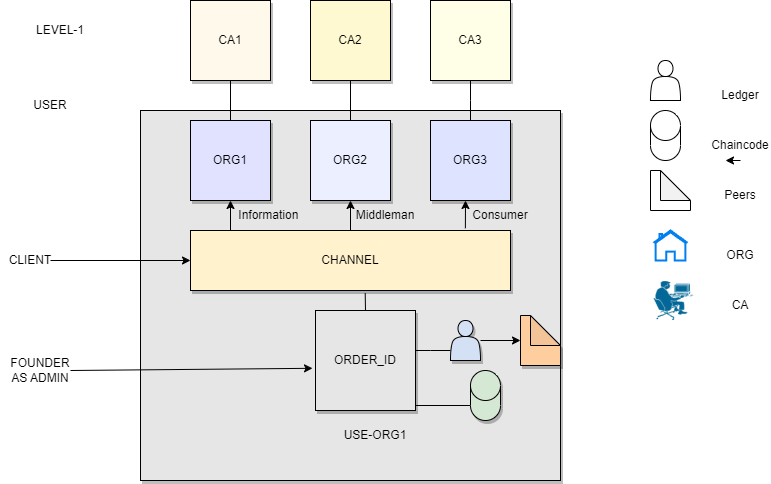
\includegraphics[width=0.9\textwidth]{Chapters/Chapter_5/figures/figure5_1.png}
  \caption{Hyperledger Fabric network Architecture }
  \label{fig:figure5_1}
  \end{figure}

\noindent The Fabric network comprises three organizations (Manufacturer, Middle Men, and Consumer) with five peers, one orderer, 
and one channel. Each organization has its own Fabric CA for managing digital certificates. The network uses Fabric CA as 
the Certificate Authority for secure authentication and authorization. The peers maintain a copy of the shared ledger and 
execute chain code for smart contracts. The Orderer validates and orders transactions, ensuring consistency. The Fabric 
network with Fabric CA provides a secure, transparent, and efficient solution for managing operations.

\begin{itemize}
  \item Admin: all the organization.
  \item Manufacturer: Org1.
  \item Middleman: Org2.
  \item Consumer: Org3.
  
\end{itemize}
    
% ----------------------------
% Scope for Future Work
% ----------------------------

\subsection{Membership and Access Control}
\begin{figure}[htbp]
  \centering
  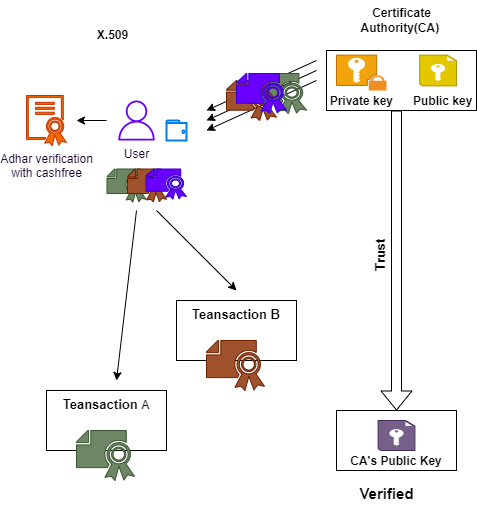
\includegraphics[width=0.9\textwidth]{Chapters/Chapter_5/figures/x.509.png}
  \caption{X.509 Identity Management }
  \label{fig:figure5_2}
  \end{figure}
\noindent \ref{fig:figure5_2} shows that there is a CA that issues a certificate to the user, and this X.059 certificate has multiple attributes whenever 
the user performs a transaction, it signs using this certificate and also checks for Aadhar verification status. Any other entity 
in the system that can view these transactions will be able to see their attributes, thereby knowing that the transaction was 
performed by the particular user to ensure trustworthy of each user in the network.

\subsection{Machine Learning}
\noindent 
The developed solution presents a machine learning (ML) model for detecting the freshness of fruits using a Convolutional Neural Network (CNN) algorithm. The model is trained using TensorFlow, an open-source library for deep learning and machine learning tasks, and is supported by other libraries such as NumPy, Pandas, and Matplotlib for data handling, data cleaning, and visualization. The dataset used for training the model is imported, and its length is verified to be 10901. The model is trained with a sequential model using different layers, including convolutional, activation, dropout, max pooling, flattening, and dense, each serving a specific function in the training process. Keras, a popular library for building neural networks, is used to create the final layers of the CNN model.
\par The model is compiled with the Adamax optimizer, a commonly used optimizer in ML models. During training, the data is traversed multiple times using epochs, with an epoch value of 30 in this case. A validation-data of validation-generator with verbose 1 used and a batch size of 15 is used in the model training process. The proposed approach combines various libraries, algorithms, and tools to develop an ML model for detecting the freshness of fruits based on their condition, which can be beneficial in tracking the quality of products in supply chains. The solution contributes to the expanding body of literature on blockchain applications by providing an effective, dependable, secure, and decentralized trace and track solution using ML and blockchain technologies.
\begin{figure}[ht]
  \centering
  \begin{minipage}[b]{0.4\linewidth}
    \centering
    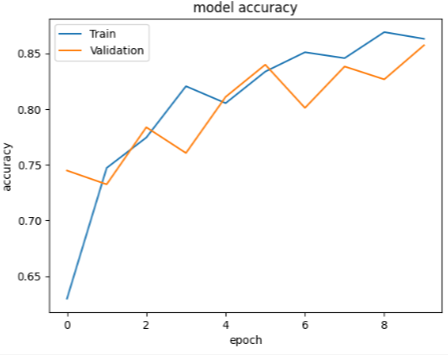
\includegraphics[width=\linewidth]{Chapters/Chapter_5/figures/model_accurecy.png}
    \subcaption{Model Accurecy}
  \end{minipage}
  \hfill
  \begin{minipage}[b]{0.4\linewidth}
    \centering
    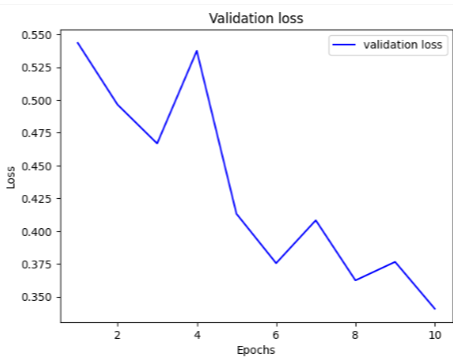
\includegraphics[width=\linewidth]{Chapters/Chapter_5/figures/validationloss.png}
    \subcaption{Validation loss}
  \end{minipage}
  \caption{Main caption}
  \label{fig:figure5_3}
  \end{figure}
  
  % \begin{figure}[ht]
  %   \centering
  %   \begin{minipage}[b]{0.7\linewidth}
  %     \centering
  %     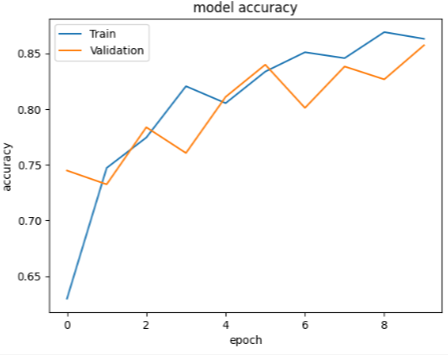
\includegraphics[width=\linewidth]{Chapters/Chapter_5/figures/model_accurecy.png}
  %     \subcaption{Model Accuracy}
  %   \end{minipage}
  
  %   \vspace{0.5cm} % Adjust the vertical space between the images
  
  %   \begin{minipage}[b]{0.4\linewidth}
  %     \centering
  %     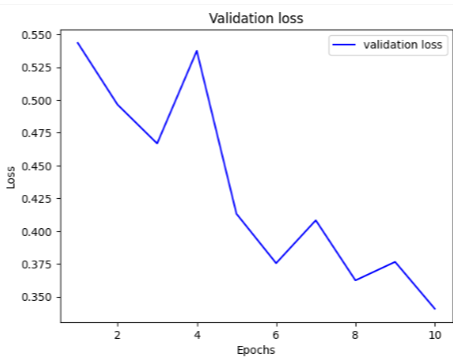
\includegraphics[width=\linewidth]{Chapters/Chapter_5/figures/validationloss.png}
  %     \subcaption{Validation Loss}
  %   \end{minipage}
    
  %   \caption{Main Caption}
  %   \label{fig:figure5_3}
  % \end{figure}
  
  
  
  
  
  
  
\noindent \ref{fig:figure5_3} (a) shows the training accuracy and Validation accucy.Train graph shows the overall model’s Training accuracy and validation accuracy shows the Subset of the training data .It is seen that with each epoch Model is giving more accuracy also validation accuracy too. Validation accuracy is calculated by using subset of the whole 
Training dataset.The final accuracy of the Model is found to be 88.5\%.
\ref{fig:figure5_3} (b) shows the output result that our model  provides.It can be seen That our model is providing us the correct
output.For a rotten Fruit it predicts the fruit as rotten and for a fresh it predicts as fresh.



 
% Chapter Template

\chapter{Implementation}\doublespacing % Main chapter title

\label{Chapter6} % Change X to a consecutive number; for referencing this chapter elsewhere, use \ref{ChapterX}

\lhead{Chapter III. \emph{Implementation}} % Change X to a consecutive number; this is for the header on each page - perhaps a shortened title

% ----------------------------
% Introduction
% ----------------------------

\section{Implementation}
This chapter describes the Implementation based on the study conducted by \textbf{Last Name et al.} on the topic \textbf{ "Article Title Article Title Article Title Article Title Article Title Article Title" } which was published in \ldots \ldots journal (Volume xx, number x).


\textit{Last Name. First Name, Last Name. First Name, ”Article Title Article Title Article Title Article
Title, vol. xx, no. xx, pp. xxx–xxx, 2022.}

% ----------------------------
% Brief outline of the study
% ----------------------------

\subsection{Brief Outline of the study}
\lipsum[22-25]


% ----------------------------
% Problem Statement
% ----------------------------

\section{Problem Statement}
Nullam molestie elit eu dolor. Nullam bibendum, turpis vitae tristique gravida, quam sapien tempor lectus, quis pretium tellus purus ac quam. Nulla facilisi: 

\begin{itemize}

  \item Nullam bibendum, turpis vitae tristique gravida, quam sapien tempor lectus, quis pretium tellus purus ac quam.
  
  \item Cibendum, turpis vitae tristique gravida, quam sapien tempor lectus, quis pretium tellus purus ac quam.
  
  \item Turpis vitae tristique gravida, quam sapien tempor lectus, quis pretium tellus purus ac quam. 
  
\end{itemize}

% ----------------------------
% Objective of the Study
% ----------------------------

\section{Objective of the Study}
 Morbi non felis ac libero vulputate fringilla. Mauris
libero eros, lacinia non, sodales quis, dapibus porttitor, pede. Class aptent taciti sociosqu ad litora torquent per conubia nostra, per inceptos hymenaeos:

\begin{itemize}

  \item Sodales quis, dapibus porttitor, pede. Class aptent taciti sociosqu ad litora torquent per conubia nostra, per inceptos hymenaeos.
  
  \item Lacinia non, sodales quis, dapibus porttitor, pede. Class aptent taciti sociosqu ad litora torquent .
  
\end{itemize}


% ----------------------------
% Methodology
% ----------------------------

\section{Methodology}
\lipsum[33]


% ----------------------------
% Study Location Selection
% ----------------------------

\subsection{Study Location Selection}
\lipsum[14] The selected sites and their configurations are shown in Figure \ref{fig:figure6_1}.

\begin{figure}[ht]
\centering
\begin{minipage}[b]{\linewidth}
  \centering
  \includegraphics[width=0.4\linewidth]{Chapters/Chapter_3/figures/Image3_1a.PNG}
  \subcaption{Plot1 with a single image (Image by pencil parker from Pixabay)}
\end{minipage}

\begin{minipage}[b]{\linewidth}
  \centering
  \includegraphics[width=0.4\linewidth]{Chapters/Chapter_3/figures/Image3_1b.PNG}
  \subcaption{Plot2 with a single image (Image by pencil parker from Pixabay)}
\end{minipage}
\caption{Main caption}
\label{fig:figure3_1}
\end{figure}









% ----------------------------
% Data Collection Strategy
% ----------------------------

\subsection{Data Collection Strategy}
\lipsum[4-5]

% ----------------------------
% Data Extraction
% ----------------------------

\subsection{Data Extraction and Coding}
\lipsum[8]

% ----------------------------
% Methodology Adopted for the Analysis
% ----------------------------

\subsection{Methodology Adopted for the Analysis}
\lipsum[3]

% ----------------------------
% Study Observations
% ----------------------------

\section{Study Observations}
Sed commodo posuere pede. Mauris ut est. Ut quis purus. Sed ac odio. Sed vehicular hendrerit sem. Duis non odio. Morbi ut dui. Sed accumsan risus eget odio. In hac habitasse platea dictumst. 

\begin{itemize}

  \item Morbi ut dui. Sed accumsan risus eget odio. In hac habitasse platea dictumst. Pellentesque non elit. Fusce sed justo eu urna porta tincidunt. Mauris felis odio, sollicitudin sed, volutpat a, ornare ac, erat.
  
  \item Sed commodo posuere pede. Mauris ut est. Ut quis purus. Sed ac odio. Sed vehicular hendrerit sem.
  
  \item Pellentesque non elit. Fusce sed justo eu urna porta tincidunt. Mauris felis odio, sollicitudin sed, volutpat a, ornare ac, erat Sed commodo posuere pede. Mauris ut est. Ut quis purus. Sed ac odio. Sed vehicular hendrerit sem.
  
\end{itemize}

% ----------------------------
% Study Limitations
% ----------------------------

\section{Study Limitations}
\lipsum[7]

% ----------------------------
% Practical Implications
% ----------------------------

\section{Practical Implications}
\lipsum[9]





 
% Chapter Template

\chapter{Results and Conclusion}\doublespacing % Main chapter title

\label{Chapter7} % Change X to a consecutive number; for referencing this chapter elsewhere, use \ref{ChapterX}

\lhead{Chapter vii. \emph{Results}} % Change X to a consecutive number; this is for the header on each page - perhaps a shortened title


% --------------------------------
% Study Summary
% --------------------------------

\section{Results}

\begin{figure}[htbp]
  \centering
  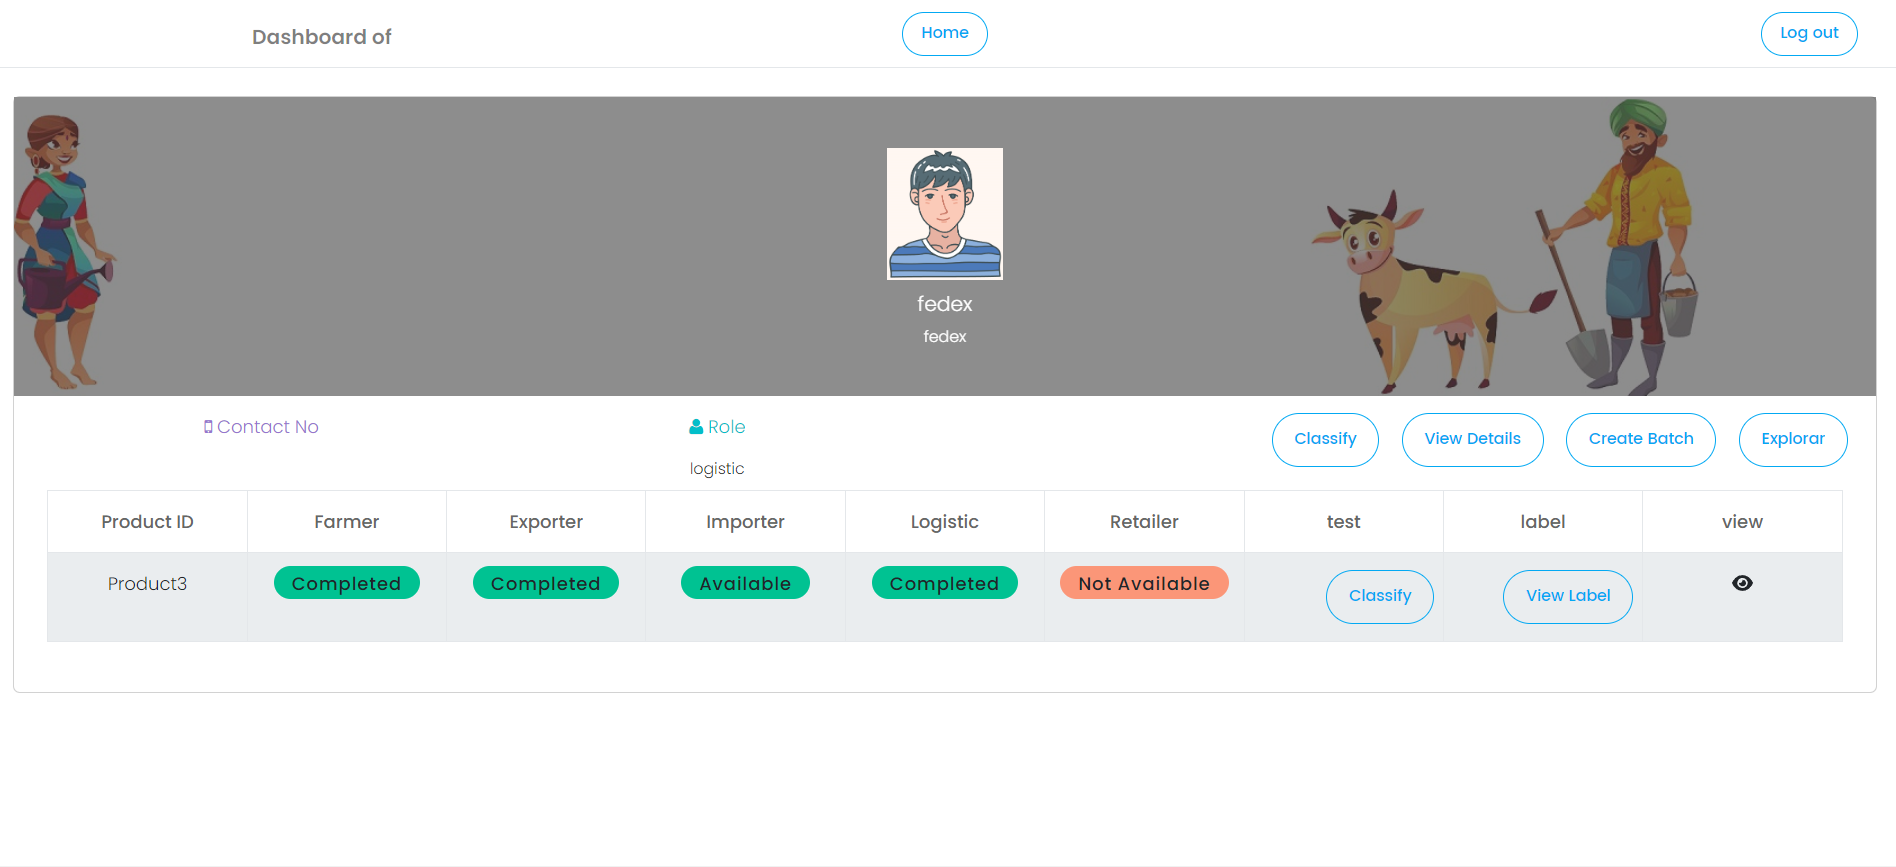
\includegraphics[width=0.9\textwidth]{Chapters/Chapter_7/images/User_interface.png}
  \caption{User Interface }
  \label{fig:figure7_1}
  \end{figure}
\noindent {The Results obtained from  our project is shown with different diagrams provided below\par}
\noindent{The provided user dashboard interface shown in Figure \ref{fig:figure7_1} offers a visually appealing and user-friendly layout for managing products within a supply chain system. Here's a description of the various sections and functionalities:
\begin{itemize}
   \item User Information Section:
   \begin{itemize}
      \item At the top of the dashboard, there is a background image with an overlay.
      \item Within the overlay, the user's profile picture, name, and address are displayed.
      \item If the user has uploaded a profile picture, it is shown; otherwise, a default image is used.
   \end{itemize}
   \item User Details Section:
   \begin{itemize}
      \item Below the user information, there are sections displaying the user's contact number and role within the system.
      \item These details provide quick access to essential user information.
   \end{itemize}
   
   \item Action Buttons:
   \begin{itemize}
      \item The dashboard includes three action buttons: "Explore," "Create Batch," and "View Details."
      \item Clicking the "Explore" button takes the user to a page for exploring products.
      \item The "Create Batch" button opens a dialog or form for creating a new batch of products.
      \item The "View Details" button allows users to access more detailed information about the system.
   \end{itemize}
   \item Product Classification Component:
   \begin{itemize}
      
      \item A component related to product classification is present on the dashboard.
      \item This component likely provides options or tools for classifying products based on specific criteria.
   \end{itemize}
   \item Product Overview Table:
   \begin{itemize}
      
      \item The main section of the dashboard features a table presenting an overview of the products.
      \item Each row in the table represents a specific product and contains several columns.
      \item The columns include the product ID and the parties involved in the supply chain, such as farmers, exporters, importers, logistic providers, and retailers.
      \item There are also columns labeled "test," "label," and "view."
   \end{itemize}
   \item Dynamic Content and Interactions:
   \begin{itemize}

\item The content in the columns of the table dynamically changes based on the product's status and role within the supply chain.
\item Different labels or status indicators, such as "Completed," "Processing," or "Not Available," are displayed to represent the current stage or availability of the product at each role.
\item Users can interact with the table by clicking on specific elements.
\item For example, clicking on the "View" column triggers an action to view more detailed information about the selected product.
\end{itemize}
\end{itemize}
In summary, this user dashboard provides an intuitive interface for managing products within a supply chain system. It offers easy access to user information, various functionalities for product management, and a comprehensive overview of products and their statuses.\par }
\begin{figure}[ht]
  \centering
  \begin{minipage}[b]{0.6\linewidth}
    \centering
    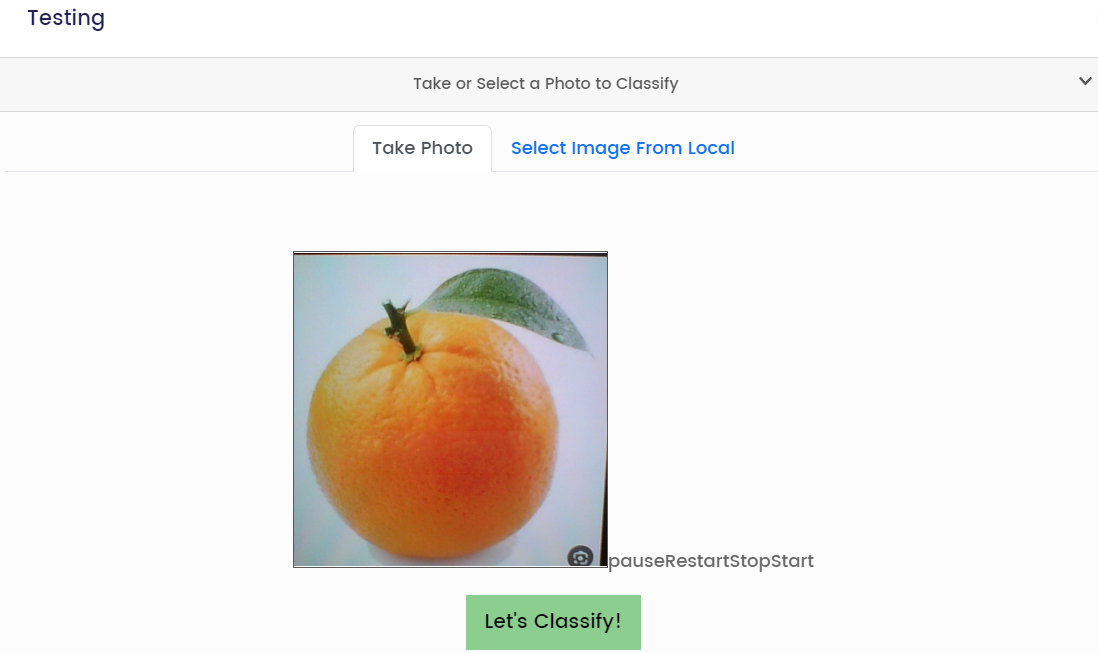
\includegraphics[width=\linewidth]{Chapters/Chapter_7/images/quality_check.png}
    \subcaption{Quality Check}
  \end{minipage}

  \vspace{0.5cm} % Adjust the vertical space between the images

  \begin{minipage}[b]{0.6\linewidth}
    \centering
    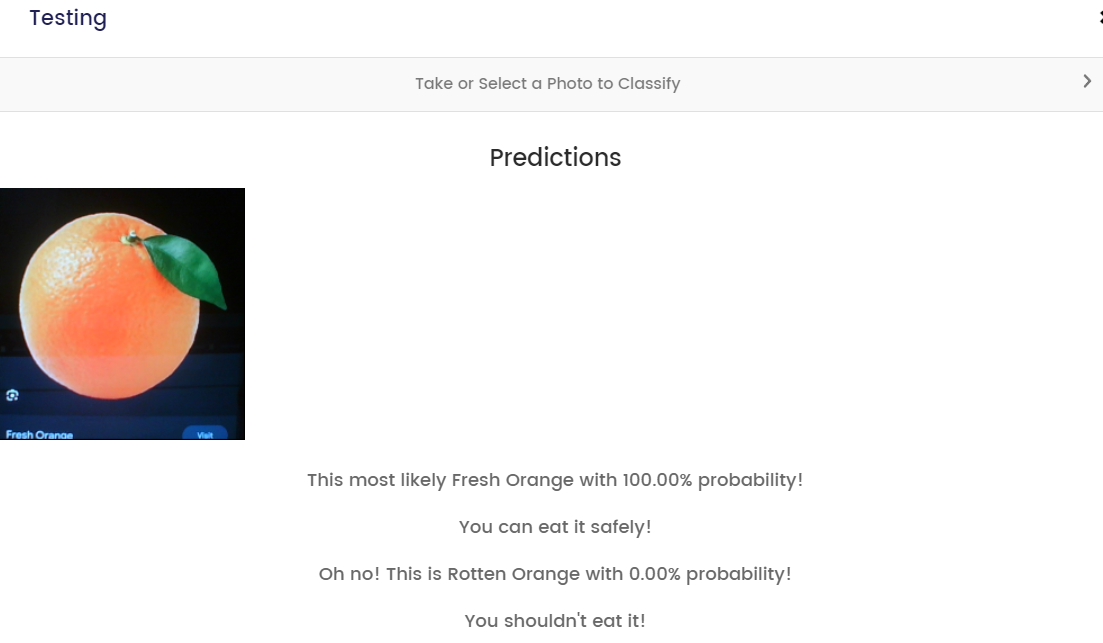
\includegraphics[width=\linewidth]{Chapters/Chapter_7/images/quality_check_result.png}
    \subcaption{Quality Check results}
  \end{minipage}
  
  \caption{Model Output}
  
  \label{fig:figure7_2}
\end{figure}
\noindent {Whenever an user wants to check whether the quality of the product is good or bad he can check that using an ML model,after checking the model is giving output as fresh if the fruit is in good condition and if not then the model is giving output as rotten.\par}
\noindent{The first diagram Figure \ref{fig:figure7_2}(A) is used to show how we can show the product to our camera sensor and after clicking on the let's clearift button it gives the result shown in the second diagram Figure i.e.\ref{fig:figure7_2}(B)}








\begin{figure}[htbp]
    \centering
    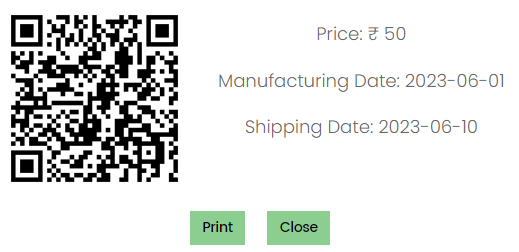
\includegraphics[width=0.7\textwidth]{Chapters/Chapter_7/images/Screenshot.png}
    \caption{Product Label }
    \label{fig:figure7_3}
    \end{figure}
\noindent {The product label shown in Figure \ref{fig:figure7_3} will provide the details of the product like the price,manufacturing date,shipping date etc.Also user can get a printed invoice of the price details\par}
\begin{figure}[htbp]
    % \centering
    \raggedright %
    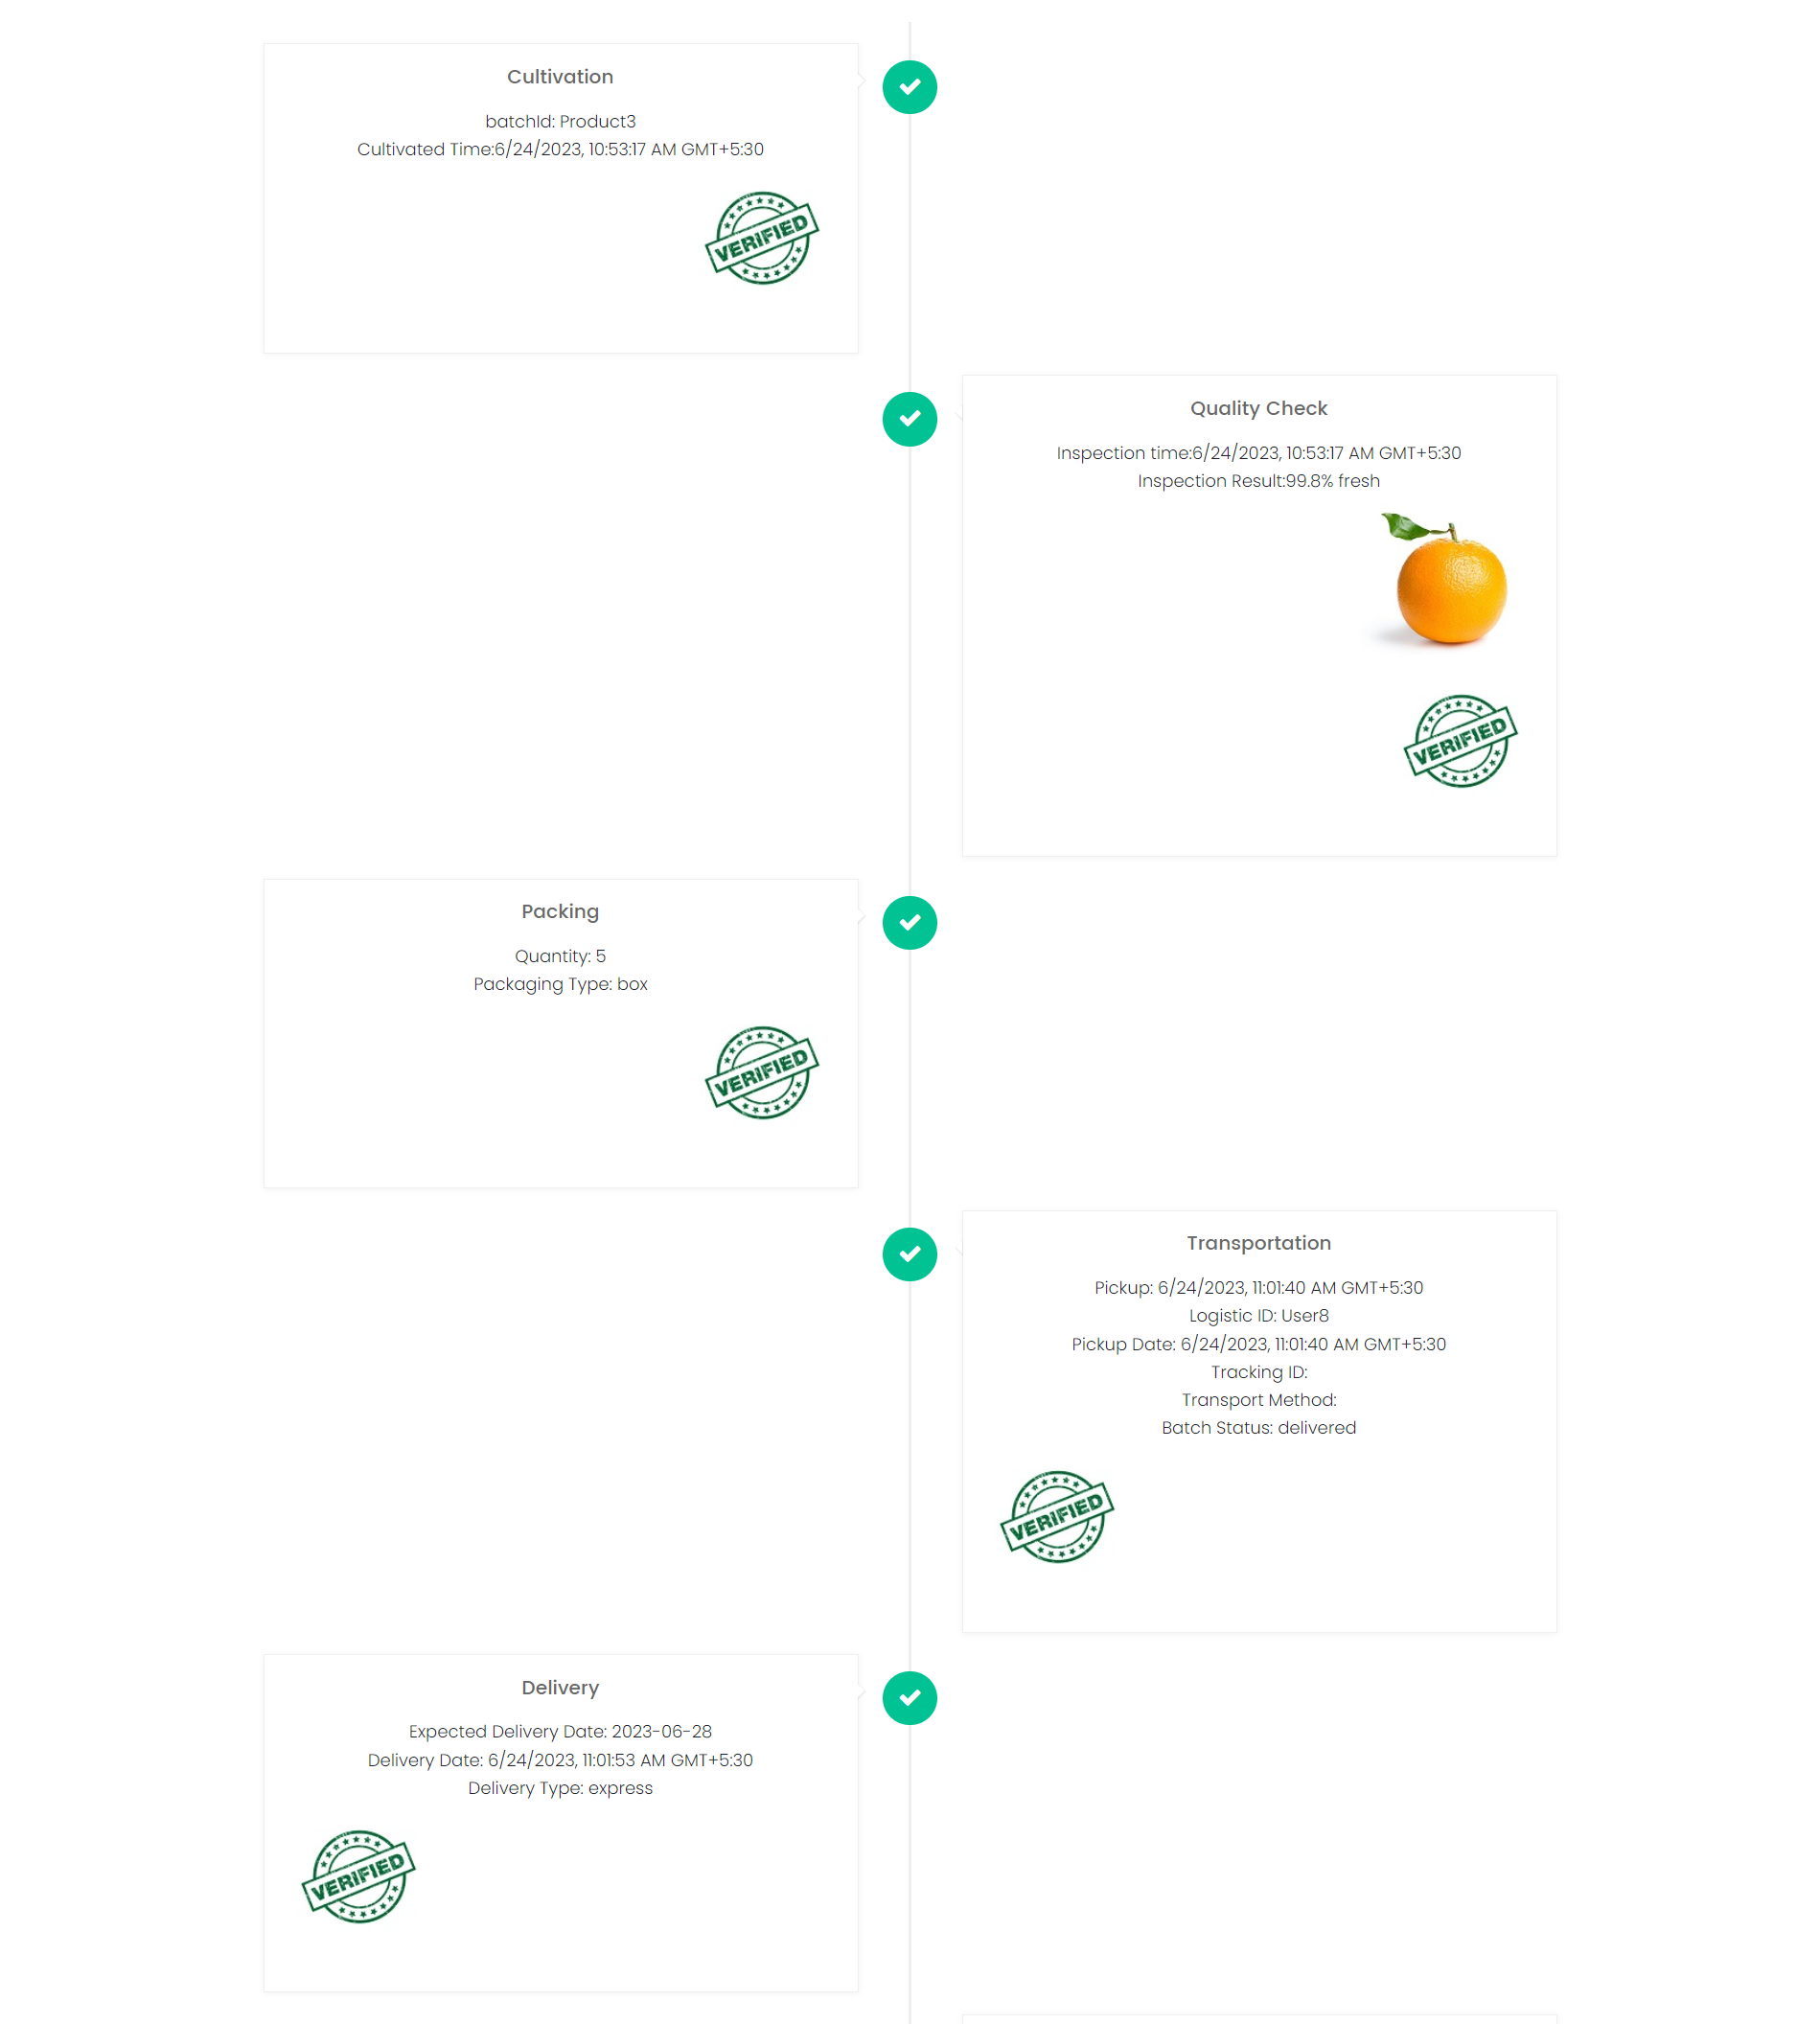
\includegraphics[width=1.2\textwidth]{Chapters/Chapter_7/images/veified.png}
    \caption{Product Timeline}
    \label{fig:figure7_4}
    \end{figure}
\noindent{The product timeline displayed in  Figure \ref{fig:figure7_4}  represents the progress and various stages of a product lifecycle in a supply chain system. The timeline showcases the different activities and events that occur during the cultivation, packaging, transportation, delivery, and marketing of a batch.

Here is a breakdown of the different sections in the batch timeline:

Cultivation: This section displays information related to the cultivation process. It includes details such as the batch ID, cultivation time, and a verification status.

Quality Check: This section represents the quality inspection stage. It shows the inspection time, inspection result, and verification status.

Packing: In this section, information about the packaging process is presented. It includes details like quantity, packaging type, and a verification status.

Transportation: This section focuses on the transportation of the batch. It provides information about the logistics involved, including the logistic ID, pickup date, tracking ID, transport method, and verification status.

Delivery: This section showcases the delivery stage of the batch. It includes details such as the expected delivery date, actual delivery date, delivery type, and verification status.

Marketing: This section represents the marketing activities related to the batch. 

Distribution: The last section,  display information about the distribution of the batch to consumers or retailers.

Each section in the timeline is presented with a timeline badge that indicates the status of that particular stage. A green badge with a checkmark represents a successful completion, while a red badge with an "X" indicates a failure or incomplete stage.

Overall, the batch timeline provides a visual representation of the product journey through the different stages of the supply chain, allowing users to track and monitor its progress.}
% \noindent{ The first diagram is used to show how we can show the fruit to our camera sensor and after clicking on the let's clearift button it gives the result shown in the second diagram i.e.Quality Check Results}
\vspace*{0.5cm}
\vspace*{0.5cm}
\section{Conclusion}
\noindent{In conclusion, a noteworthy development in the agriculture sector is the adoption of a blockchain-based farming system that combines supply chain management with machine learning algorithms to track and evaluate food quality. By ensuring transparency, traceability, and improved food safety, this novel concept transforms conventional farming methods.

The solution gives customers access to an immutable, decentralised ledger of all farming and supply chain activity by utilising blockchain technology. The ability to trace the path of their food from farm to table gives consumers the power to make knowledgeable decisions about the products they buy. The blockchain's immutability shields users from fraud, manipulation, and the introduction of fake items into the supply chain.
The system is further advanced because to the incorporation of machine learning models. These algorithms are able to analyse a variety of factors, including farming methods, environmental factors, and quality indicators, to evaluate the overall quality of the food by utilising enormous amounts of data. This enables prompt responses to reduce these risks and aids in the identification of potential hazards like contamination or spoiling. In the end, it makes sure that consumers have access to high-quality, safe food products.
All parties involved will profit greatly from the farming system's integration of blockchain and machine learning. Farmers may boost productivity, allocate resources more efficiently, and obtain insights into their farming practises. Distributors and retailers may increase customer trust while reducing waste and managing their inventory more effectively. On the other side, customers can relax knowing that they have open access to information on the food they eat.

Overall, the  blockchain-based farming system augmented by machine learning system raises industry standards for food safety, supply chain effectiveness, and consumer empowerment. It is a key step towards creating a food ecosystem that is safer and more sustainable, and it encourages everyone to take responsibility for their actions.









}
% ----------------------------
% Methodology
% ----------------------------

\section{Future Scope}
\noindent {The integration of blockchain-based farming systems with supply chain management and machine learning algorithms opens up a promising future for the agriculture industry. Here are some potential futurescopes for this innovative concept:

1. Enhanced Food Safety and Quality Assurance: As the technology continues to evolve, the integration of blockchain and machine learning can further enhance food safety and quality assurance measures. Advanced sensors and IoT devices can be integrated into the system to continuously monitor and collect real-time data on various parameters such as temperature, humidity, and soil conditions. This data can be analyzed by machine learning models to detect potential risks and ensure proactive interventions, thereby minimizing the occurrence of foodborne illnesses and maximizing food quality.

2. Expansion of Traceability and Certification: The blockchain-based farming system can extend its traceability capabilities by incorporating smart contracts and digital certifications. Smart contracts can automatically verify and enforce compliance with specific farming standards and regulations. Digital certifications, issued through blockchain, can provide a trustworthy and immutable record of organic, fair trade, or other specific product attributes. This expansion of traceability and certification will empower consumers with even more information about the origin, production practices, and authenticity of the food they purchase.

3. Integration with IoT and Automation: The integration of the farming system with the Internet of Things (IoT) and automation technologies holds immense potential. IoT devices such as drones, sensors, and autonomous machinery can be used to collect data, monitor crop health, and automate farming processes. These devices can interface with the blockchain system, recording and verifying data in real-time, while machine learning algorithms can analyze the data to optimize resource allocation, predict crop yields, and enable more efficient farming practices.

4. Consumer Engagement and Education: The blockchain-based farming system can serve as a platform for consumer engagement and education. Through mobile applications or web interfaces, consumers can access detailed information about the food they consume, including farming practices, environmental impact, and nutritional profiles. Educational resources, such as tutorials on sustainable farming or healthy eating, can be integrated into the system, promoting awareness and empowering consumers to make conscious food choices.

5. Global Collaboration and Standards: The adoption of blockchain-based farming systems can foster global collaboration and the establishment of common standards in the agriculture industry. By providing a transparent and decentralized platform, stakeholders from different regions and countries can collaborate, share best practices, and collectively work towards sustainable and efficient food production. This collaboration can lead to the development of globally recognized standards for farming practices, supply chain management, and quality assurance, promoting harmonization and trust across international markets.

In conclusion, the future of blockchain-based farming systems combined with supply chain management and machine learning is promising. With continued advancements and innovations, we can expect improved food safety, expanded traceability, increased automation, enhanced consumer engagement, and global collaboration in the agriculture industry. This technology-driven future holds the potential to create a more sustainable, transparent, and secure food ecosystem for the benefit of all stakeholders involved.}

 



% %\break
% \clearpage % Start a new page
% %\thispagestyle{plain}

% \addtotoc{Study Limitations and Scope for Future Work} % Add the "Scope for future work" page entry to the Contents

% {\addtocontents{toc}{\vspace{1em}} % Add a gap in the Contents, for aesthetics
% \lhead{\emph{Study Limitations and Scope for Future Work}} 

% \centerline{\LARGE \textit{{Study Limitations and Scope for Future Work}}}
% \vspace{3em}
% Like any other study, this study is also not without limitations due to shortage of resources and field setting. The study limitations and future research scopes are presented below.

% \begin{itemize}
%     \item The pedestrians' road crossing behaviour was observed only during non-peak hours (11 am to 2 pm) to avoid the influence of traffic police (forcibly stopping pedestrian from signal violation). Thus, future research should include both peak and non-peak hours to study pedestrians' unsafe road crossing behaviour. 
    
%     \item In signal violation research social and non-social factors were studied on one-way crosswalks. In future research the same approach could be extended to two-way crosswalks.
    
%     \item Research involving the interaction between variables (demographics of leader and follower pedestrian violating signal) could help in better understanding the pedestrian signal violation risk-taking behaviour.
    
%     \item The current study did not account for the driver's behaviour such as yielding behaviour, speeding and rush driving into consideration. Future research involving these explanatory variables can provide better insight into pedestrian risk-taking behaviour.
    
%     \item To get an initial understanding of pedestrian distracted road crossing behaviour in developing countries like India, similar to past studies, the present study also considered crosswalks with one step crossing (three one-way crosswalks). The current study methodology can be extended to two-way divided streets in terms of two-step crossing to understand more complex crossing behaviour, where pedestrians could use mobile phones in the first step of crossing (start to median) and might not use on the second step (median to end) or vice-versa. 
    
%      \item Future research should also investigate how pedestrians utilise their hearing senses to perceive their environments (especially pedestrians who are holding the phone or texting and not wearing headphones). This would provide a better understanding of how situational awareness is reduced by mobile phone use or if pedestrians are relying on senses other than sight to inform them of traffic conditions.
    
%     \item The current distraction study only measured influence of various distractors in road crossing behaviour. In future research, distracted unsafe road crossing behavioural estimates could be incorporated with Level of Service measure to identify unsafe signalized intersection crosswalks.
    
%     \item Combining objective observational data (on all stages of pedestrian road crossing) with subjective data (questionnaire survey) from the same observed pedestrian would provide a better understanding of human factors involved in crossing behaviour at signalised intersection crosswalks. 
    
    
%     \item The observations under the current study were made only based on one city level data, which may restrict the scope of the conclusions drawn from the current study. Thus, future studies need to extend the methodology to  a wider variety of intersections, and samples with a more diverse category of signalised and unsignalised intersections over different Indian provinces (commercial, residential, and educational) to make findings more generalised.
% \end{itemize}

% Although there are several possibilities for future research in this domain, the results obtained from this study can be of great help for researchers, policymakers, design practitioners, and engineers. These findings will also be useful for designing better interventions and reducing unsafe crossing behaviour. 


% }

\clearpage % Start a new page
%----------------------------------------------------------------------------------------
%	THESIS CONTENT - APPENDICES
%----------------------------------------------------------------------------------------

\addtocontents{toc}{\vspace{2em}} % Add a gap in the Contents, for aesthetics

\appendix % Cue to tell LaTeX that the following 'chapters' are Appendices

% Include the appendices of the thesis as separate files from the Appendices folder
% Uncomment the lines as you write the Appendices

% % Appendix Template

% \chapter{APPENDIX CHAPTER TITLE} % Main appendix title

% \label{AppendixA} % Change X to a consecutive letter; for referencing this appendix elsewhere, use \ref{AppendixX}

% \lhead{Appendix A. \emph{APPENDIX CHAPTER TITLE}} % Change X to a consecutive letter; this is for the header on each page - perhaps a shortened title

% % Appendix Template

% \chapter{APPENDIX CHAPTER TITLE} % Main appendix title

% \label{AppendixB} % Change X to a consecutive letter; for referencing this appendix elsewhere, use \ref{AppendixX}

% \lhead{Appendix B. \emph{APPENDIX CHAPTER TITLE}} % Change X to a consecutive letter; this is for the header on each page - perhaps a shortened title

% % Appendix Template

% \chapter{APPENDIX CHAPTER TITLE} % Main appendix title

% \label{AppendixC} % Change X to a consecutive letter; for referencing this appendix elsewhere, use \ref{AppendixX}

% \lhead{Appendix C. \emph{APPENDIX CHAPTER TITLE}} % Change X to a consecutive letter; this is for the header on each page - perhaps a shortened title


%\input{Appendices/AppendixD}

\addtocontents{toc}{\vspace{2em}} % Add a gap in the Contents, for aesthetics

\backmatter

%----------------------------------------------------------------------------------------
%	BIBLIOGRAPHY
%----------------------------------------------------------------------------------------

\label{References}

\lhead{\emph{References}} % Change the page header to say "Bibliography"
% \usepackage{natbib}
%\renewcommand{\refname}{References}
\renewcommand\bibname{References}
% \bibliographystyle{elsarticle-harv} % Use the "custom" BibTeX style for formatting the Bibliography
\bibliographystyle{plain} % Use the "custom" BibTeX style for formatting the Bibliography
% \setcitestyle{year,open={((},close={))}}

\bibliography{references} % The references (bibliography) information are stored in the file named "Bibliography.bib"

\newpage
% Appendix Template

% \chapter{List of Publications} % Main appendix title

% \label{LOP} % Change X to a consecutive letter; for referencing this appendix elsewhere, use \ref{AppendixX}

% \lhead{\emph{List of Publications}} % Change X to a consecutive letter; this is for the header on each page - perhaps a shortened title


    
\newpage
\include{Biography}


\end{document}  
